
\begin{TP}[Méthode géométrique de calcul du PGDC]

\partie{Découverte de la méthode}
Dans cette partie, nous allons illustrer le calcul du PGDC de 18 et 22 par une figure géométrique.\\[0.5em]
On commence par construire un rectangle $ABCD$ tel que $AB = 18$ et $BC = 22$. On construit ensuite le carré $ABEF$. Dans la surface restante représentée par le rectangle $ECDF$, on peut placer quatre carrés de côté $EC$. On construit ensuite le carré $JLMF$ et on constate que la surface restante est l'intérieur d'un carré : \textcolor{C2}{$LKDM$}.
\begin{center} 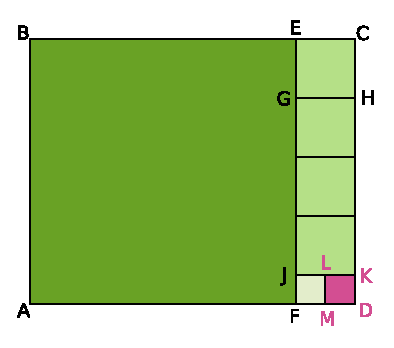
\includegraphics[width=5.7cm]{methode_geometrique} \end{center}

\begin{enumerate}
 \item Chaque membre du groupe reproduit cette figure en choisissant un carreau ou 1 cm comme unité ;
 \item Chaque membre calcule le PGDC de 18 et 22 ;
 \item À quelle longueur correspond le PGDC de 18 et 22 ?
 \end{enumerate}
 
\partie{Quelques autres exemples}

\begin{enumerate}
 \item Chaque membre détermine le PGDC de 12 et 45 par la méthode géométrique (sur une feuille à petits carreaux) ;
 \item Chaque membre vérifie son résultat en calculant le PGDC de 12 et 45 par la méthode des soustractions successives ;
 \item Chaque membre choisit un nombre entre 10 et 20 et un autre nombre entre 40 et 50. Il donne ses deux nombres à son voisin de droite qui doit déterminer leur PGDC par la méthode géométrique (sur une feuille à carreaux).
 \end{enumerate}
 
\end{TP}

%%%%%%%%%%%%%%%%%%%%%%%%%%%%%%%%%%%%%%%%%%%%%%%%%%%%%%%%%%%%%%%%%%%

\begin{TP}[Dans le coeur des micros]

\partie{Parlons chiffre}

En informatique, on utilise seulement des 0 et des 1 pour coder les nombres. On travaille avec un système de numération binaire.

\begin{center}
\begin{tabularx}{0.7\linewidth}{|X|X|c|}
\hline
Écriture binaire & Écriture décimale & Lien entre les deux écritures \\ \hline
1 & 1 & $1\cdot 2^0$ \\ \hline
10 & 2 & $1\cdot2^1+0\cdot 2^0$ \\ \hline
11 & 3 & $1\cdot2^1+1\cdot 2^0$ \\ \hline
100 & 2 & $1\cdot2^2+0\cdot 2^1+0\cdot 2^0$ \\ \hline
\end{tabularx} \\
\end{center}

\begin{enumerate}
 \item Observez bien la table de correspondance précédente puis déterminez l'écriture en binaire des entiers inférieurs à 10 ; \label{NbsEntMultDivis_engroupe}
 \item Reproduisez la feuille de calcul suivante sur un tableur : \\[1em]
 \begin{center}
 \begin{tabularx}{0.7\linewidth}{|X|X|X|X|X|X|X|X|X|}
 \hline
 \rowcolor{Gris2} & A & B & C & D & E & F & G & H \\ \hline
 \cellcolor{Gris2} 1 & \multicolumn{5}{l|}{Nombre en binaire}  & & & \\ \hline 
 \cellcolor{Gris2} 2 & 0 & 1 & 1 & 1 & 1 & 1 & 0 & 1 \\ \hline
 \cellcolor{Gris2} 3 & \multicolumn{7}{l|}{Nombre en écriture décimale} & \ldots  \\ \hline 
 \end{tabularx} \\
 \end{center}
 
 \vspace{1em}
 
 Programmez en H$3$ le calcul nécessaire pour obtenir l'écriture décimale d'un nombre en binaire.
  \end{enumerate}
  
  
 \partie{La table ASCII}
 L'unité d'enregistrement en informatique est le \textbf{bit}, symbolisé par un 0 ou un 1. Un \textbf{octet} correspond à une suite de huit bits, par exemple 0100 1101.
 
 \begin{enumerate}
 \item Combien de nombres peut-on écrire avec un octet ? \\[0.75em]
Pour coder la centaine de caractères présents sur un clavier, on les numérote de 0 à 255 et on les code à l'aide d'un octet. La table qui permet de mettre en correspondance un caractère et le nombre entre 0 et 255 s'appelle la \textbf{table ASCII}. Récupérez-la sur Wikipedia.
 
 \item Retrouvez l'écriture décimale du nombre 0100 0001. À quelle lettre correspond-il ?
 \item À l'aide de la question \textbf{\ref{NbsEntMultDivis_engroupe}}, retrouvez l'écriture en binaire des codes des autres lettres de l'alphabet.\\[0.75em]
Choisissez alors quatre mots de moins de dix lettres, codez-les en binaire puis demandez aux autres groupes de les retrouver. Faites de même avec les mots qui vous auront été donnés.
 \end{enumerate}
\end{TP}

%%%%%%%%%%%%%%%%%%%%%%%%%%Mise en page

\vspace*{3cm}

\phantom{Pour sauter une ligne}

%%%%%%%%%%%%%%%%%%%%%%%%%%%%%%%%%%%%%%


